\chapter{Pair Alignment}
\section{Alignment}
Alignment refers to the proper positioning or state of adjustment of parts (as of a mechanical or electronic device) in relation to each other.
It is a fundamental technique in bioinformatics and often it represents the first step in many evolutionary and functional studies. Errors in alignment tend to amplify in later computational stages.\\
In general we talk about alignment of sequences and there are essentially two reasons for which it is very useful:
\begin{itemize}
	\item \textbf{Studying function}, sequences that are similar probably have similar functions;
	\item \textbf{Studying evolution}, similarity is mostly indicative of common ancestry;
\end{itemize}
\image{img/ancestor.png}{Common ancestor example}{0.5}

\subsection{Homology}
Two important concepts used in bioinformatic are related to the notion of \textbf{homology} and \textbf{analogy}.\\

\textbf{A is Homologous to B} if they are related by divergence from a common ancestor. Then we can find another division of this family:
\begin{itemize}
	\item Paralogues, different but related functions in one organism.
	\item Orthologues, same function in different organisms.
\end{itemize}

\textbf{A is Analogous to B} if they gave a similar function but possibly different origins. Different sequence with the same structure may have common ancestor, instead different sequence with different structure may be convergent to evolution.\\

Now we define $4$ operators that can change a sequence:
\begin{figure}[h]
	\begin{minipage}[t]{0.5\linewidth}
		\centering
		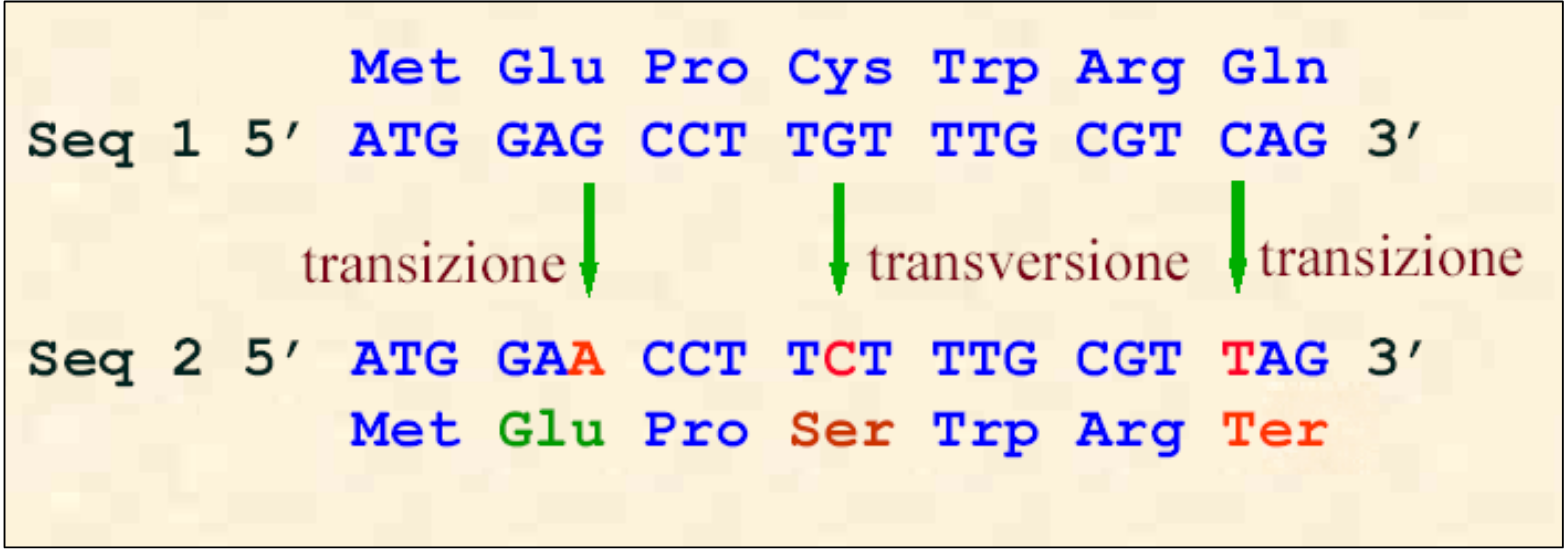
\includegraphics[width=0.9\textwidth]{img/mutation.png}
		\caption{Mutation operator.}
		\label{f1}
	\end{minipage}
	\hspace{0.1cm}
	\begin{minipage}[t]{0.5\linewidth} 
		\centering
		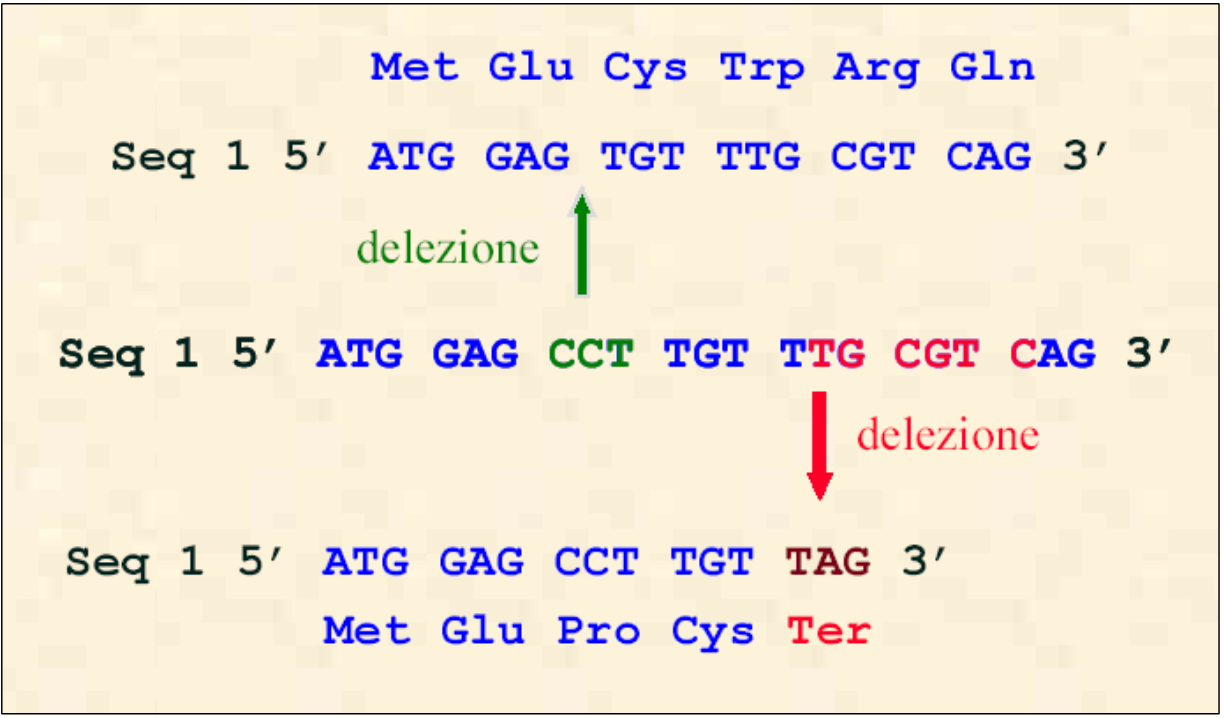
\includegraphics[width=0.9\textwidth]{img/deletions.png}
		\caption{Deletion operator.}
		\label{f2}
	\end{minipage}        
\end{figure} 

\begin{figure}[h]
	\begin{minipage}[t]{0.5\linewidth}
		\centering
		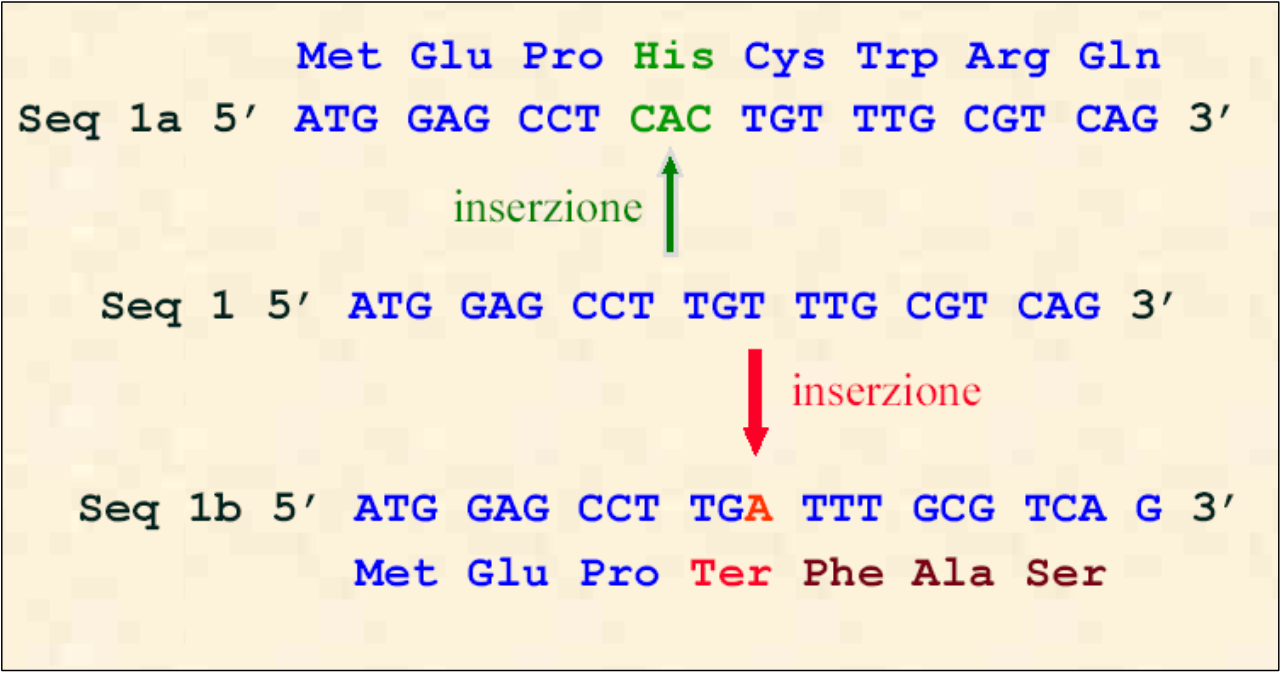
\includegraphics[width=0.9\textwidth]{img/insertions.png}
		\caption{Insertion operator.}
		\label{f1}
	\end{minipage}
	\hspace{0.1cm}
	\begin{minipage}[t]{0.5\linewidth} 
		\centering
		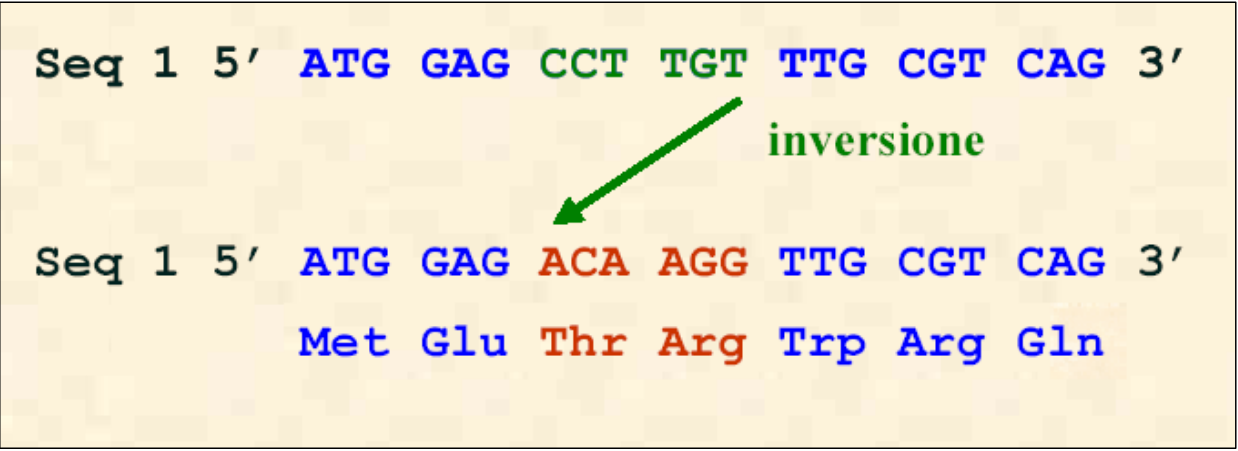
\includegraphics[width=0.9\textwidth]{img/inversions.png}
		\caption{Inversion operator.}
		\label{f2}
	\end{minipage}        
\end{figure} 
\image{img/omologia.png}{Homologous sequences}{0.5}


\section{Sequence Alignment}
Sequence alignment would require the identification of the correct location of \textit{deletions} and \textit{insertions} that have occurred in either of the two lineages since their divergence from a common ancestor. This never happens, it is impossible, but we can check for the \textbf{maximal parsimony hypothesis}, which is an optimal criterion under which the phylogenetic tree that minimizes the total number of character-state changes is to be preferred.\\
When we talk about alignment we should take in consideration different things like: type of alignment, allowing gaps, score system, algorithm and evaluation of the results.

\subsection{Type of Alignment - 1.}
Two main types of alignment:
\begin{itemize}
	\item \textbf{Global alignment}, compares the whole sequence $A$ with the whole sequence $B$. It is used in comparative and evolutionary studies.
	
	\item \textbf{Local alignment}, determines if sub-segments of one sequence ($A$) are present in another ($B$). It finds its greatest utility in database searching and retrieval. 
\end{itemize}
When we have biological sequences that are distant from each other it could be difficult to obtain a correct alignment in regions of low similarity. Local alignment avoids such regions altogether and focuses on those with a positive score, i.e. those with an evolutionary conserved signal of similarity.

\subsection{Type of Alignment - 2.}
Sequence alignment may be divided into two categories:
\begin{itemize}
	\item \textbf{Pairwise alignment}, alignment of two sequences. This problem has \textit{exact solution}.
	\item \textbf{Multiple-sequence alignment}, alignment of three or more sequences. It is not exact solved, but there exist some approximate (heuristic) solutions.
\end{itemize}

\subsection{Gaps}
There are \textbf{internal} and \textbf{terminal} gaps.
\image{img/gaps.png}{Type of gaps.}{0.6}
\begin{itemize}
	\item \textbf{Internal}, they are located inside the string and they may indicate that a deletion or an insertion has occurred in one of the two lineages.
	\item \textbf{Terminal}, they are located on the external sides of the string and they may indicate missing data.
\end{itemize}

\subsection{Methods of alignment}
Alignment can be performed in different ways:
\begin{itemize}
	\item Manual
	\item Dot matrix
	\item Exact alignment
	\item Heuristic (word methods)
\end{itemize}

\subsubsection{Manual Alignment}
When there are few gaps and the two sequences are not too different 
from each other, a reasonable alignment can be obtained by 
\textbf{visual inspection}. 

\subsubsection{Dot matrix}
The two sequences are written out as column and row heading of two-dimensional matrix. A \textbf{dot} is put in the dot-matrix plot at a position where the nucleotides in the two sequences are identical. Then we can distinguish $4$ different cases:
\begin{itemize}
	\item \textbf{match}, indicated by a diagonal step through a dot. (Diagonal step from a cell to another one which have a dot)
	
	\item \textbf{mismatch}, indicated by a diagonal step through an empty element of the matrix. (Diagonal step from a cell to another one which is empty)
	
	\item A \textbf{gap} in the sequence used in column (on the top of the matrix), indicated with a vertical step
	
	\item A \textbf{gap} in the sequence used in row (on the left of the matrix), indicated with a horizontal step.
\end{itemize}
\image{img/dot_matrix.png}{Dot matrix between two biological sequences.}{0.4}
An interesting property of the dot matrix is that it allows to find also palindrome strings looking for opposite diagonals.

The main problem of this visualization tool is that when we have long sequences the dot matrix became not easy to understand. With long sequences (like DNA sequences) the matrix becomes cluttered. In order to improve its readability the \textbf{sliding window} technique is adopted, which is based on the idea of collapsing the dots in the original dot matrix. The sliding window procedure consists on defining a matrix $k\times k$ and starting from the first position on the dot matrix check if there are at least $h$ dots inside the window. In case of positive match a new dot in the center of the window is included in the new dot matrix. Otherwise no dots are included. The parameters $k$ and $h$ are called \textbf{windows size} and \textbf{stringency} respectively. The main advantage of this procedure is that changing the values of $k$ and $h$ we can project the original dot matrix in different scales and have different views on data (\textbf{trial-and-error}).

\image{img/dotMatrixSliding3.png}{Dot matrix example with sliding window $k = 3$ and $h = 2$.}{1}

\textbf{Advantages} of dot matrix:
\begin{itemize}
	\item It is simple to implement.
	\item Trial-and-error procedure to have different views on data. It can be useful since it may unravel information on the evolution of sequences or it may be used to compare one sequence to itself and study repetitions. 
\end{itemize}

\textbf{Disadvantages} of dot matrix:
\begin{itemize}
	\item Expensive for large sequences analyses.
	\item It may not identify the best possible alignment.
	\item Qualitative view, either match or mismatch, no quantification with a similarity score.
\end{itemize}

\subsubsection{Exact and Heuristic}
The true alignment between two sequences is the one that reflects accurately the evolutionary relationship between the sequences. Since the \textbf{true alignment} is unknown, in practice we look for the \textbf{optimal alignment}, which is the one in which the number of mismatches and gaps are minimized according to a certain criteria (depending on the score).\\

In order to determine an optimal alignment we need to choose a scoring system, which comprises a \textbf{gap penalty} and a \textbf{scoring matrix} $M(a,b)$ that specifies the score for each type of match (a = b) or mismatch (a $\neq$ b). 

Extra: The units in a scoring matrix may be the nucleotides in DNA or RNA sequences, the codons in protein-coding regions, or the amino acids in protein sequences.\\

Mismatch and gap penalties should be \textit{inversely proportional to the frequencies} with which changes occur. Scoring matrices are based on the \textit{additive property of the score} meaning that it implies position independence and the score can be calculated by scrolling the string.
\newpage
\subsubsection{Scoring matrices for DNA}
DNA scoring matrices are usually simple, since all mismatches are given the same penalty:
$$M(a,b) = \begin{cases}
>~0 & \text{if}~a = b\\ 
\leq~0 & \text{if}~a \neq b\\
\end{cases}$$
In more complicated matrices a distinction may be made and each type of mismatch may be penalized differently.

\subsubsection{Scoring matrices for Aminoacids}
For aminoacids we can distinguish among different matches and mismatches. Example: a mismatched pair consisting of $Leu~\&~lle$, which are very similar biochemically to each other, may be given a lower penalty than a mismatched pair consisting of $Arg~\&~Glu$, which are very dissimilar from each other.

\subsection{Gap Penalties}
\textbf{Gap penalty} (or cost) is a factor (or a set of factors) by which the gap values (numbers and lengths of gaps) are multiplied. The gap penalties are based on our assessment of how frequent different types of \textit{insertions} and \textit{deletions} occur in evolution in comparison with the frequency of occurrence of point substitutions.\\
The gap penalty may have two components:
\begin{itemize}
	\item a gap-opening penalty
	\item a gap-extension penalty
\end{itemize}

In literature we have different systems for gap penalty:
\begin{itemize}
	\item \textbf{Fixed gap-penalty system}, example $0$ gap costs.
	\item \textbf{Linear gap-penalty system}, the gap cost is calculated by multiplying the gap length $g$ by a costant $d$: $\gamma(g) = -gd$.
	\item \textbf{Affine score}, it distinguishes a gap-opening cost $d$ and a gap-extension cost $e$: $\gamma(g) = -d - (g-1)e$, with $e~<~d$.
	
	\item \textbf{Logarithmic gap-penalty system}, the gap-extension penalty increases with the logarithm of the gap length (slower).
\end{itemize}

\image{img/logGap.png}{Gap penalty.}{0.6}

\image{img/effectOfGap.png}{Effect of gap penalties on amino acid alignment.}{0.8}

\subsection{Scoring matrices: Log-odds ratios}
A scoring matrix is a table of values that describes the probability of an amino acid pair to occur in an alignment. The values in a scoring matrix are \textbf{log rations of two probabilities},  meaning that:
\begin{itemize}
	\item One is the random probability (denominator);
	\item The other is the probability of a empirical pair occurrence (numerator);
\end{itemize}
The scores are logarithms of probability ratios, hence they can be added to give a meaningful score for the entire alignment. \textit{The more positive the score, the better the alignment}.\\
Let $x = x_1 \dots x_n$ and $y = y_1 \dots y_n$ be the pair of sequences to align (for simplicity no gap), it is possible to define:

\paragraph{Probability of the random alignment:} $P(x,y|R) = \Pi_{i = 1,n}{q_{xi}}~ \Pi_{j = 1,n}{q_{y_j}}$  \\
where $q_{xi},~q_{yj}$ are the probabilities of the symbols $x_i$ and $y_j$.

\paragraph{Probability of being correlated:} $P(x,y|M) = \Pi_{i = 1,n}{q_{x_iy_i}}$  \\

\textbf{Ratio}: $\frac{(P(x,y|M))}{P(x,y|R)} = \frac{\Pi_{i = 1,n}q_{x_iy_i}}{\Pi_{i = 1,n}q_{x_i} \Pi_{j=1,n}q_{y_j}} = \Pi_{i = 1,n}\Big[\frac{q_{x_iy_i}}{q_{x_i}q_{y_i}}\Big]$
where $q_{ix},~q_{yj}$ are the probabilities of the symbols $x_i$ and $y_j$.\\

\textbf{Log}: $\sum_{i = 1,n} \log(\frac{q_{x_iy_i}}{q_{x_i}q_{y_i}})$ in general multiplied by $10$ to get an integer.
\newpage
\subsection{Empirical substitution matrices}
\begin{itemize}
	\item \textbf{PAM} (Percent/Point Accepted Mutation) matrices assume a model where amino acid substitutions, observed at great evolutionary distances, it is the sum of many independent mutations. Hence, the \textit{PAM scores express the likelihood that the pairing of a pair of amino acids is due to homology rather than to the case.} PAM matrices are built through homologous sequences that represents only the 1\% of accepted mutations, where for "accepted" it is meant mutations that don't alter the protein function.\\
	\textbf{PAM1} matrix is the amount of evolutionary change that yields one substitution in 100 amino acids residues. To derive a mutational probability matrix for a protein sequence that has 	undergone N percent accepted mutations, a \textbf{PAM-N} matrix, the	PAM-1 matrix is multiplied by itself N times.

	\item \textbf{BLOSUM} (BLOcks SUbstitution Matrix) matrices do not make any homology assumption: the considered blocks are obtained by direct observation of the proteins having similar functions.
\end{itemize}

PAM matrices work but they have some disadvantages:
\begin{itemize}
	\item Assumed regular time in evolution;
	\item Assumed same evolutive speed for different species;
	\item No gap is considered;
	\item The phylogenetic tree is inferred;
	\item Simplifying assumptions in the computation of the scores: symmetry, reversibility and independence from position;
\end{itemize}

BLOSUM matrices are based on local alignments ("blocks" or conserved amino acid patterns). All BLOSUM matrices are based on observed alignments and they are not extrapolated from comparisons of closely related proteins. BLOSUM\textit{n} is based on sequences that are at most $n$ percent identical.

\paragraph{Comparison between PAM and BLOSUM.} Both of them are scoring matrices that define the penalties to apply in case of mismatch, but they tend to favor different behaviors. In particular PAM tends to favor homology and BLOSUM tends to favor functionalities.

\chapter{Pair alignment - Methods}
\section{Approximated Pattern Matching}
Consider the match between a text $T$ and a pattern $P$ with the possibility of having \textit{errors} both in the pattern and in the text. We can define a \textbf{similarity/distance between strings}. Ex: $aab$ is similar to $aac$? We need a \textbf{threshold} to distinguish when the comparison is meaningful.\\
Having a similarity measure between strings can be useful for different applications like: finding typos in texts, signal recovery with noise, finding similar strings in DNA or proteins, comparing two sequences. \\

Difference between strings is given by in terms of length and of symbols that they have. We can think that difference between strings can be expressed in the type and number of transformation is required to transform one string into the other one. There are $4$ operations that can be applied to modify strings:
\begin{itemize}
	\item \textbf{Insertion}, insert a symbol into the string; $Ex:~ aaa~\rightarrow~aaba$
	\item \textbf{Deletion}, eliminate a symbol from the string: $Ex:~ aaba~\rightarrow~aaa$
	\item \textbf{Substitution}, substitute a symbol with another one in the string; $Ex:~ aaba~\rightarrow~aaca$
	\item \textbf{Transportation}, switch the order of two adjacent symbols in the string; $Ex:~ aaba~\rightarrow~aaab$
\end{itemize}
These operations are associated to a \textbf{cost}, that can be:
\begin{itemize}
	\item They may have the same cost (\textit{constant});
	\item Different cost for each operation;
	\item Even a different cost for each symbol (\textit{penalty matrices}).
\end{itemize}

\section{Distance between two strings}
Let $A$ and $B$ be two strings, their \textbf{distance} $d(A,B)$ is the minimal cost of a sequence of operations which transform $A$ into $B$. If there is not such a sequence of transformations the cost is infinite $(\infty)$.
$$Ex:~A~=~POLITE,~B=~PLATE$$
$$\text{POLITE}~\rightarrow \text{delete(2)},~ \text{substitution(3,A)}~\rightarrow~\text{PLATE}$$
This is the minimal sequence of operations considering, and if we fix that the cost of each operation is $1$ then the distance is $2$.\\
On the rest of this section we are going to propose different distance metrics for comparing strings.

\subsection{Hamming Distance}
It permits only substitutions for computing distance between strings. It is symmetric and not transitive: $\text{if }|A|~=~|B|,~ 0\leq d(A,B) \leq |A|$.\\

$\text{Ex: X = aaaccd, Y =abcccd}$\\
$d(X,Y)~=~2 \quad \text{since at least two substitutions are necessary.}$

\subsection{Levenshtein(Edit) Distance}
It permits the usage of more transformation operation respect to the hamming distance, which consider only substitutions. The edit distance, in fact, takes in consideration insertions, deletions and substitutions. It is symmetric and has the following property:
$$0 \leq d(A,B) \leq max(|A|,|B|)$$
$$\text{EX: X = aaaccd, Y = abccd}$$
$$d(X,Y) = 2 \quad \text{since at least a substitution and a deletion are necessary.}$$

\subsection{Episode Distance}
It permits only insertions and it isn't symmetric. Since it consider only insertions it is possible that $A$ and $B$ cannot match through transformation, meaning that $d(A,B)= \infty$. Otherwise in the other cases we have that $d(A,B)=|B|-|A|$.

$$\text{EX: X = aaccd, Y = abbaccd}$$
$$d(X,Y) = 2 \quad \text{since two insertions are necessary.}$$

\section{Similarity between two strings}
Let $d$ be a distance and $e$ be an error threshold, then we can define a \textbf{similarity relation between strings}, $\sim_e$:
$$A\sim_eB \qquad d(A,B)\leq e$$
This concept extends the equality relation between strings and in general it is not transitive and it may not be symmetric.


\section{Pair Alignments}
An alignment between a string $A$ with $n$ symbols and a string $B$ with $m$ symbols is an array $L$ of dimension $2\times max(n,m)$, in which:
\begin{itemize}
	\item the first row contains the symbols of $A$ or $\varepsilon$;
	\item the second row contains the symbols of $B$ or $\varepsilon$;
\end{itemize}
so that by eliminating $\varepsilon$ one can obtain $A$ and $B$ again. 

\image{img/globalAlignment.png}{Global Alignment.}{0.6}
From the previous example we have seen that for two strings we can have multiple available alignments. In general we have a fixed number of alignments:
$$\binom{n+m}{min(n,m)} = \frac{(n+m)!}{n!m!}\approx \sqrt{\frac{n+m}{2\pi nm}}\times \frac{(n+m)^{(n+m)}}{n^n\times m^m}$$
where $n$ and $m$ are the lengths of the two sequences to be aligned.

\subsection{Optimal Alignment}
An optimal alignment is an alignment in which the \textbf{distance} between the two strings is \textbf{minimal} (or the similarity is maximal).
\image{img/optimalAlignment.png}{Optimal Alignment example.}{0.6}

\subsection{Back to Approximated Pattern matching}
The problem of the Longest Common Subsequence (LCS) of two given sequences consists on: given a similarity relation between strings $\sim_e$ it is possible to search for strings similar to a pattern $P$ in a text $T$. We need a method to compute the minimal distance/maximal similarity between two strings (the optimal alignment) and a method to search the substrings similar to $P$ in $T$.


\subsection{Exact Optimal Alignment Algorithms}
Optimal alignment can be reached with different algorithms:

\paragraph{Dynamic programming.} Let $A$ and $B$ two strings of length $n$ and $m$, respectively, then we define $D(i,j)$ as the edit distance between $A[1\dots i]$ and $B[1\dots j]$. In other words $D(i,j)$ denotes the minimum number of edit operations needed to transform $A[1\dots i]$ into $B[1\dots j]$.\\
Edit operations are:
\begin{itemize}
	\item insertion of a character;
	\item deletion of a character;
	\item substitution of a character;
\end{itemize}
Hence the edit distance of $A$ and $B$ is the value $D(n,m)$. We use a dynamic programming approach to compute $D(n,m)$, which is composed by three main components:
\begin{enumerate}
	\item \textbf{Recurrence relation}, establish a recursive relation between the value of $D(i,j)$ with $i,j$ positive, and values of $D$ for index pairs smaller than $i$ and $j$;
	\item \textbf{Tabular computation}, uses the recursive relation to efficiently compute $D(n,m)$. There can be applied two types of approaches. \textit{Top-down approach} using recursion, but it is not efficient. The \textit{bottom-up approach} first compute $D(i,j)$ for the smallest possible values and then compute $D(i,j)$ for all the choices of $i$ and $j$.
	\item \textbf{Traceback}, once all values of $D$ have been computed, extract an optimal solution;
\end{enumerate}

\image{img/editDistanceInductive.png}{Edit distance: inductive definition.}{0.5}

\paragraph{Needleman-Wunsch Algorithm}
The Needleman-Wunsch algorithm allows to build the edit distance table given in input two strings $A$ and $B$, with dimension $n$ and $m$. It assumes that the cost of each operation is $1$ and produces in output a table $D$, $n\times m$, containing the values of the \textbf{edit distance} and the links.  $D$ is inductively defined with respect to the indexes.

\image{img/needlemanWunsch.png}{Needleman-Wunsch Algorithm to build the edit distance table.}{0.5}

When the value of $D[i,j]$ is computed, set a pointer (one or more) from $D(i,j)$ to :
\begin{itemize}
	\item $D[i-1, j-1]$ if $D[i,j] = D[i-1,-1] + f(i,j)$;
	\item $D[i, j-1]$ if $D[i,j] = D[i,j-1] + 1$ (horizontal step);
	\item $D[i-1, j]$ if $D[i,j] = D[i-1,j] + 1$ (vertical step);
\end{itemize}
For cells in row $0$ or column $0$ set a pointer to the only possible direction. The pointers allow for an easy recovery of an optimal edit transcript from $A$ to $B$: simply follow any path of pointers from cell $D[n,m]$ to cell $D[0,0]$:
\begin{itemize}
	\item a vertical step corresponds to aligning a symbol in $A$ with a gap in $B$;
	\item a horizontal step corresponds to aligning a symbol in $B$ with a gap in $A$;
	\item a diagonal step corresponds to a match or a mismatch.
\end{itemize}

\image{img/computingPointers.png}{Example of computing pointers.}{0.5}

The complexity of N-W:
\begin{itemize}
	\item Space: $S(nm)$ which is required to store $D$.
	\item Time for building $D$: $O(nm)$;
	\item Time for tracing back an optimal alignment: $O(n+m)$; 
\end{itemize}

\image{img/needleman-wunsch.png}{Example of Needleman-Wunsch Algorithm.}{0.6}

\paragraph*{Inductive definition of the similarity score.} The similarity score can be obtained also through an inductive definition where $D[i,j]$ is the score of the optimal alignment between $A[1 \dots i]$ and $B[1 \dots j]$.\\
\image{img/inductive_definition}{Inductive definition of the similarity score.}{0.55}
Thanks to this definition it is possible to define the N-W algorithm.

\subsection{Semiglobal Alignments}
Semiglobal alignment is useful when one sequence is short (for example a gene sequence) and the other is very long (for example a chromosome sequence). In that case, the shortest sequence should be globally aligned but only a local alignment is desired for the long sequence. The shortest sequence is aligned through the introduction of external gaps that can allow the pre-computation of specific rows/columns of the resulting table.
\image{img/semiglobal1}{Semiglobal Alignments.}{0.7}
\image{img/semiglobal2}{Semiglobal Alignments.}{0.7}
The application of this improvement makes possible for us to determine the following algorithm:
\image{img/edit_distance_inductive}{Semiglobal Alignment: Edit Distance Inductive Definition.}{0.55}

\subsection{Approximated Pattern Matching}
It is possible to notice the fact that semiglobal alignment is similar but not equal to an approximated pattern matching, indeed, the pattern is usually much shorter than the text.\\
We can consider a problem where:
\begin{itemize}
	\item \textbf{Input:} a pattern $P$ of size $m$, a text $T$ of size $n$ and an error threshold $\delta$ (Each operation costs 1 and match costs 0).
	\item \textbf{Output:} a table $D$ of size $m \times n$ containing the edit distance.
\end{itemize}
With these premises, it is possible to define the approximated pattern matching algorithm through the building of the distance table $D$.
\image{img/approximated_pattern_matching}{Approximated pattern matching: building of the distance table.}{0.55}
This algorithm produces the following table:
\image{img/approximated_pattern_matching_table}{Table created with the approximated pattern matching algorithm.}{0.55}
In order to find possible occurrences of $P$, we can notice that any $D[m,j] \leq \delta$ corresponds to an approximated occurrence of $P$. In a more detailed way:
\image{img/occurences_P}{Procedure used to find approximated occurrences of $P$.}{0.55}

\subsection{Comparison between global/local alignment.} Global and local alignment are used for different purposes indeed:
\begin{itemize}
	\item \textbf{Global alignment} is used for sequences comparison.
	\begin{center}
		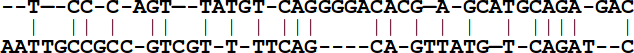
\includegraphics[width=0.5\textwidth]{img/global}
	\end{center}
	\item \textbf{Local alignment} allows to find conserved motifs.
	\begin{center}
	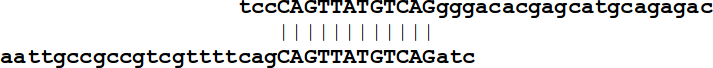
\includegraphics[width=0.5\textwidth]{img/local}
	\end{center}
\end{itemize}

\paragraph*{Smith-Waterman Algorithm.} The initial scoring matrix of S-W enables the alignment  of  any segment of one sequence to an arbitrary position in the other sequence. It can do this because of the fact that no negative score is assigned in the scoring system.\\
This algorithm has the following properties:
\begin{itemize}
	\item It enables local alignment.
	\item When any element has a score lower than 0, it means that the sequences up to this position have no similarities. This element will then be set to 0 to eliminate influence from previous alignment.
	\item In this way, calculation can continue to find alignment in any position afterwards.
\end{itemize}
The distance table $D$ is created through the following procedure:
\image{img/SW1}{S-W: similarity score between two sequences.}{0.6}
As it is possible to see, the procedure is applicable also when scores can be negative. The S-W algorithm has the following input/output:
\begin{itemize}
	\item \textbf{Input:} two sequences to be aligned \textbf{A} and \textbf{B}, a threshold for the minimal score $\delta$.
	\item \textbf{Output:} a table $D$, $m \times n$, containing the values of the similarity score.
\end{itemize} 
The S-W algorithm is described as follows:
\image{img/SW2}{S-W algorithm.}{0.6}
The resulted scoring table (with match = +1, mismatch/gap=-1) can be observed below:
\image{img/SW3}{Resulting table.}{0.6}
The previous table is used in order to find local alignments. If $D[i,j] \geq \delta$ and in the next cells (adjacent lower and to the right) the score is smaller, we have a local optimal alignment. In other words, it starts from such a $D[i,j]$ and then it traverses the table towards up and left (following the pointers), up to a cell with score 0.\\
The choice of the alignments (many could be produced in general) depends on the application.
\begin{center}
	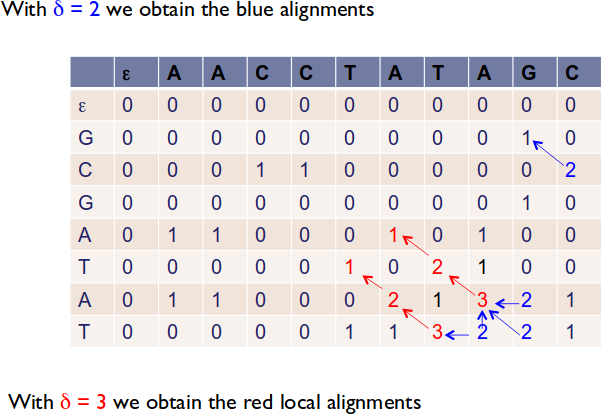
\includegraphics[width=0.73\textwidth]{img/SW4}
\end{center}

\paragraph*{Comparison between N-W and S-W.} Easily it is possible to differentiate the two algorithms according to their purposes:
\begin{itemize}
	\item \textbf{S-W} finds the segments in two sequences that have similarities.
	\item \textbf{N-W} aligns two complete sequences.
\end{itemize}
However they can be compared surely through their similarities and their differences. Both the algorithms use the concepts of a substitution matrix, a gap penalty function, a scoring matrix and a traceback process. On the other hand, they present also several differences:
\begin{table}[H]
	\centering
	\begin{tabular}{| p{2.5cm} | p{5.5cm} | p{5.5cm}|}
		\hline
		 & \textbf{S-W algorithm} & \textbf{N-W algorithm} \\
		 \hline
		 \textit{Initialization} & First row and first column are set to 0. & First row and first column are subject to gap penalty.\\
		 \hline
		 \textit{Scoring} & Negative score is set to 0. & Score can be negative. \\
		 \hline
		 \textit{Traceback} & Begin with the highest score, end when 0 is encountered. & Begin with the cell at the lower right of the matrix, end at top left cell.\\
		\hline
	\end{tabular}
	\caption{Differences between S-W and N-W.}
\end{table}

\subsection{Heuristic Methods.}
They are much faster than exact methods (N-W, S-W) that usually require a time complexity of $O(n^2)$. The drawback of these heuristic methods is that they do not guarantee to find the optimal alignment.

\paragraph*{MUMmer.} \textit{Maximal Unique Matches} (MUMs) is identified in two sequences by a generalized suffix tree. The purpose is to find the longest increasing sequences of MUMs without crossing.
\image{img/MUMs}{MUMmer representation.}{0.75}

\paragraph*{FASTA.} It is 10 times faster than S-W, it is considered as an accurate tool especially for sequences with repetitions (DNA). The algorithm is divided in the following steps:
\begin{itemize}
	\item Split the query into words (DNA ktup=4 or 6, proteins	ktup=1 or 2).
	\item Build a lookup table which shows the positions in the query for each word (\textit{indexing the query}).
	\item Build a lookup table also for the target sequence, which shows the shifts with respect to the query (\textit{indexing the target}).
	\item Determine the best similarities by comparing the shifts (\textit{Init1}: diagonals).
	\item Extend close diagonals with gaps (\textit{InitN}) like a dot-plot.
	\item Apply \textbf{Smith-Waterman} to the diagonals.  
\end{itemize}

\paragraph*{BLAST.} It stands for Basic Local Alignment Search Tool and it is 50 times faster than S-W. BLAST is the nowadays standard tool for local sequence similarity searching. It follows these steps:\\
Given a query sequence and a sequence DB:
\begin{itemize}
	\item Split the query into words of length W (4 or 3) by a \textbf{sliding window} of size W.
	\item For each word generate a list of similar words called \textbf{W-mers} with similarity score greater than T (global alignment using N-W).
	\image{img/BLAST}{BLAST step 2.}{0.5}
	\item Find good local alignments of words into DB (\textbf{seeds}) (\textbf{one hit method}). 
	\image{img/BLAST2}{BLAST step 3.}{0.5}
	\item Extend the \textbf{hit} on both sides without gap, up to a score threshold S (without applying S-W, it only recomputes the score).
	\item If the score is negative, \textbf{X} specifies how much to insist on extending the alignment.
		\image{img/BLAST3}{BLAST step 5.}{0.5}
\end{itemize}

\paragraph*{FASTA vs BLAST.} Between these two algorithms, we can find the following differences:
\begin{table}[H]
	\centering
	\begin{tabular}{| p{7cm} | p{7cm}|}
		\hline
		\textbf{FASTA} & \textbf{BLAST} \\
		\hline
		\textit{Init1} is determined through identity, hence it can miss the optimal alignment. & Generally gaps are not inserted.\\
		\hline
		It is better for DNA-RNA. & It is better for proteins (similarity, not exact match). \\
		\hline
	\end{tabular}
	\caption{Differences between FASTA and BLAST.}
\end{table}

\subsection{Results Evaluation.}
Given an alignment of a query sequence A with a sequence B with score S, it is necessary to ask what does it mean this result?\\ 
In a set of random sequences, how much is the probability to find an alignment with A with score S? (\textbf{Assessment of significance}) To determine that the similarity between two sequences is not fortuitous it is necessary to define a random population of sequences "similar" to the real one. In other words we want to check if the score of similarity S is reasonable or it is just a case in which the probability plays a noising effect. \\
For solving this purpose it is necessary to build a distribution starting from the string B. A control population can be generated by \textbf{randomizing} B in some way:
\begin{itemize}
	\item In global alignments, by applying 1000 random permutations to B;
	\item In DB search, by sampling randomly;   
\end{itemize}
Then once that the population of strings is computed we build the scoring distribution with the following steps:
\begin{itemize}
	\item Align A to each sequence in the control population;
	\item Study the score distribution;
	\item Find the obtained score $S$ and the number of cases corresponding to scores $\geq S$.
	\item We compute the \textbf{z-score} $= \frac{S-\mu}{\sigma}$. The greater it is the more valid is the similarity obtained.
\end{itemize}
In other words if the obtained score $z-score$ is distance from the average $\mu$, it means that the score obtained can be considered statically significant.

\image{img/gumber_distribution.png}{Gumber distribution over random strings.}{0.6}